\begin{figure}[h]
  \centering
  {\fbox{
      $\begin{array}{c}

         \includegraphics[width=0.9\textwidth]{fig/ProtocoloP1.png}\\

         \TEqD\ (\texttt{MOD})\\

         \progfigmed{
         defmodule EfetivacaoEmDuasFases do\\
         ~~require Oracle\\
         ~~@oracle spawn(Oracle, :listen, [])\\
         \\
         ~~@gr "<value for GR>"\\
         ~~def gr, do: @gr\\
         ~~...\\
         end\\
         \\
         EfetivacaoEmDuasFases.main(\%\{\\
         ~~estado\_gr: EfetivacaoEmDuasFases.gr\\
         ~~~~|\textgreater{} Enum.map(fn (g) -\textgreater{} \{g,
         "trabalhando"\} end)\\
         ~~~~|\textgreater{} Enum.into(\%\{  \}),\\
         ~~estado\_gt: "inicio",\\
         ~~g\_rs\_preparados: MapSet.new([]),\\
         ~~msgs: MapSet.new([])\\
         \})
         }
        
       \end{array}$
     }}
   \caption{Tradução do módulo Efetivação em Duas Fases}
   \label{fig:protocolo-ex-mod}
 \end{figure}

 \begin{figure}[h]
  \centering
  {\fbox{
      $\begin{array}{c}

         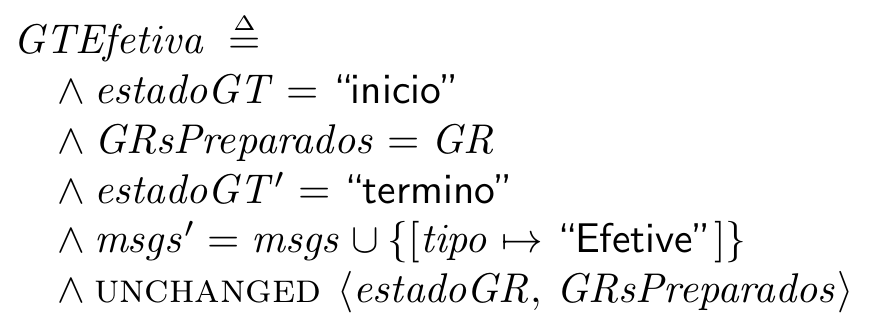
\includegraphics[width=0.6\textwidth]{fig/ProtocoloP2.png}\\

         \TEqD\ (\texttt{DEF})\\

         \progfig{
         def gt\_efetiva\_condition(variables) do\\
         ~~variables[:estado\_gt] == "inicio" and\\
         ~~~~variables[:g\_rs\_preparados] == @gr\\
         end\\
         \\
         def gt\_efetiva(variables) do\\
         ~~\%\{\\
         ~~~~estado\_gt: "termino",\\
         ~~~~msgs: MapSet.put(variables[:msgs], \%\{ tipo: "Efetive" \}),\\
         ~~~~estado\_gr: variables[:estado\_gr],\\
         ~~~~g\_rs\_preparados: variables[:g\_rs\_preparados]\\
         ~~\}\\
         end
         }

       \end{array}$
     }}
   \caption{Tradução da definição $GTEfetiva$ do protocolo}
   \label{fig:protocolo-ex-def1}
 \end{figure}

 \begin{figure}[h]
  \centering
  {\fbox{
      $\begin{array}{c}

         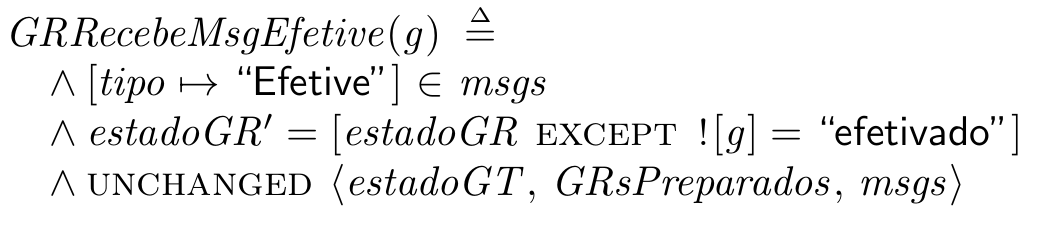
\includegraphics[width=0.7\textwidth]{fig/ProtocoloP3.png}\\

         \TEqD\ (\texttt{DEF})\\

         \progfig{
         def gr\_recebe\_msg\_efetive\_condition(variables, g) do\\
         ~~Enum.member?(variables[:msgs], \%\{ tipo: "Efetive" \})\\
         end\\
         \\
         def gr\_recebe\_msg\_efetive(variables, g) do\\
         ~~\%\{\\
         ~~~~estado\_gr: Map.put(variables[:estado\_gr], g, "efetivado"),\\
         ~~~~estado\_gt: variables[:estado\_gt],\\
         ~~~~g\_rs\_preparados: variables[:g\_rs\_preparados],\\
         ~~~~msgs: variables[:msgs]\\
         ~~\}\\
         end
         }
       \end{array}$
     }}
   \caption{Tradução da definição $GRRecebeMsgEfetive$ do protocolo}
   \label{fig:protocolo-ex-def2}
 \end{figure}

 \begin{figure}[h]
  \centering
  {\fbox{
      $\begin{array}{c}

         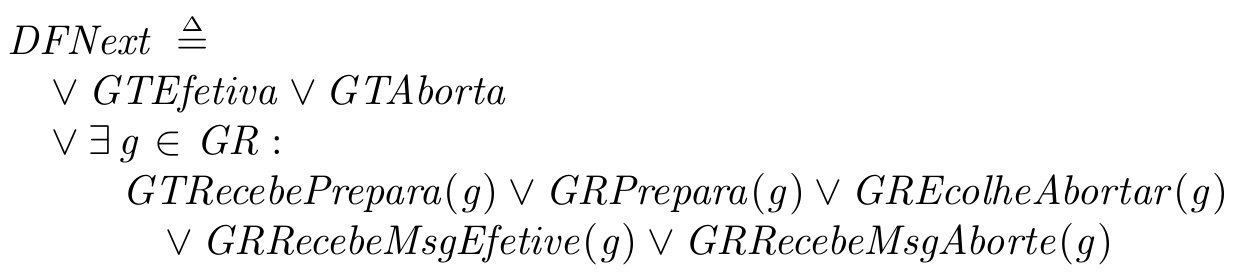
\includegraphics[width=0.7\textwidth]{fig/ProtocoloP4.png}\\

         \TEqD\ (\texttt{NEXT})\\
         \hspace*{-0.2cm}
         \progfig{
         def main(variables) do\\
         ~~IO.puts (inspect variables)\\
         \\
         ~~main(\\
         ~~~~decide\_action(\\
         ~~~~~~List.flatten([\\
         ~~~~~~~~\%\{ action:\ "GTEfetiva()",\\
         ~~~~~~~~~~~condition:\ gt\_efetiva\_condition(variables),\\
         ~~~~~~~~~~~state:\ gt\_efetiva(variables) \},\\
         ~~~~~~~~\%\{ action:\ "GTAborta()",\\
         ~~~~~~~~~~~condition:\ gt\_aborta\_condition(variables),\\
         ~~~~~~~~~~~state:\ gt\_aborta(variables) \},\\
         ~~~~~~~~Enum.map(@gr, fn (g) -\textgreater{} [\\
         ~~~~~~~~~~\%\{ action:\ "GTRecebePrepara(\#\{inspect g\})",\\
         ~~~~~~~~~~~~~condition:\ gt\_recebe\_prepara\_condition(variables, g),\\
         ~~~~~~~~~~~~~state:\ gt\_recebe\_prepara(variables, g) \},\\
         ~~~~~~~~~~\%\{ action:\ "GRPrepara(\#\{inspect g\})",\\
         ~~~~~~~~~~~~~condition:\ gr\_prepara\_condition(variables, g),\\
         ~~~~~~~~~~~~~state:\ gr\_prepara(variables, g) \}\\
         ~~~~~~~~~~~...\\
         % ~~~~~~~~~~\%\{ action:\ "GREcolheAbortar(\#\{inspect g\})",\\
         % ~~~~~~~~~~~~~condition:\ gr\_ecolhe\_abortar\_condition(variables, g),\\
         % ~~~~~~~~~~~~~state:\ gr\_ecolhe\_abortar(variables, g) \},\\
         % ~~~~~~~~~~\%\{ action:\ "GRRecebeMsgEfetive(\#\{inspect g\})",\\
         % ~~~~~~~~~~~~~condition:gr\_recebe\_msg\_efetive\_condition(variables,g),\\
         % ~~~~~~~~~~~~~state:\ gr\_recebe\_msg\_efetive(variables, g) \},\\
         % ~~~~~~~~~~\%\{ action:\ "GRRecebeMsgAborte(\#\{inspect g\})",\\
         % ~~~~~~~~~~~~~condition:\ gr\_recebe\_msg\_aborte\_condition(variables,g),\\
         % ~~~~~~~~~~~~~state:\ gr\_recebe\_msg\_aborte(variables, g) \}\\
         ~~~~~~~~] end)\\
         ~~~~~~])\\
         ~~~~)\\
         ~~)\\
         end
         }
       \end{array}$
     }}
   \caption{Tradução da função de próximo estado para o protocolo}
   \label{fig:protocolo-ex-next}
 \end{figure}
